%%%%%%%%%%%%%%%%%%%%%%%%%%%%%%%%%%%%%%%%%%%%%%%%%%%%%%%%%%%
% Chapter 1
\chapter{Introduction}\label{Ch:1}
\begin{singlespacing}
\begin{microabstract}
    The aim of this chapter is to present an overview of this thesis by first presenting the motivation for this research along with a robust business justification. A brief introduction to e-FX options and platforms is provided based on intimate industry knowledge. The chapter also outlines the research objectives, the overall framework used for learning the RFQs along with an explanation of each component in the framework. The model selection component presents a two-by-two matrix used as a foundation for this research. Finally the chapter introduces the experiments conducted along with the structure of this thesis.
\end{microabstract}
\end{singlespacing}


\section{Motivation for this research}\label{Ch1Sec1}
While machine learning is increasingly being used to support the customer purchase process in financial institutions, the use of predictive analytics is still relatively limited. For example, one of the more sophisticated applications is the robo-advisor platforms used across a number of large financial institutions such as HSBC, Fidelity, RBS and Santander. These platforms provide automated investment advice to institutional and retail customers based on their profiles. However, they do not have the predictive power to enable targeted sales actions to close the deals. This thesis explores advanced techniques for time-series predictive analytics to take these capabilities to the next level.

This work was in part inspired by the commercial opportunity in FX option sales, and in part by the philosophical debate between the classicists and the Bayesians. This study will investigate both techniques for predicting customer quote requests as well as identifying the underlying hidden market dynamics behind it. The ability to predict the next quote request will enable banks to a)~configure an offering that better meets the clients’ needs at that particular time, thus increasing sales conversion rates and b)~cross-sell or upsell other suitable products, thus increasing average order size. Further, the ability to predict the market regime within which the request is occurring (i.e., booming, flat or declining market demand), will help banks optimise pricing to achieve the sale at the best margins.

The business justification has been validated through discussions with professionals in the industry both on the sales and trading sides. Also, it should be noted that the techniques discussed here are not constrained to the banking industry and will apply in businesses in general where there is a time-series repeatable customer order aspect. Whilst these techniques have been utilised to a greater degree in the business-to-consumer retail space (e.g., Amazon, Booking.com, eBay), there have been less applications in the business-to-business space. The proof-of-concept in Finance could open up doors to many other B2B markets.


\section{Brief overview of e-FX}\label{Ch1Sec3}

\subsection{e-FX options}\label{Ch1Sec3S1}

Electronic foreign exchange (e-FX) options are a type of financial instrument known as derivatives. They are not fundamentally different to FX options (also called currency options) except that they are priced and traded electronically via digital platforms rather than by voice.
Other commonly traded e-FX products are FX spots, forwards, swaps as well as non-deliverable instruments. FX Options derivatives give the owner (purchaser) the right but not the obligation to buy (`call option`) or sell ('put option') a specified amount of one currency in exchange for another (for example EUR-USD) at a pre-agreed exchange rate or price (known as the strike price) on a specific date. The FX market is one of the largest and most liquid of options with trading volumes in trillions, which is why it was chosen for this research as a source of data. There are many different flavours of FX Options, which along with their pricing and risk management is beyond the scope of this thesis.


\subsection{e-FX trading platforms and RFQ's}\label{Ch1Sec3S1}

The foreign exchange market and in particular the FX option instrument type in the dealer-to-client market are traded electronically on single-dealer platforms (SDPs) or multi-dealer platforms (MDPs), both of which emerged in the late 1990's. SDPs are proprietary, customisable trading platforms offered by a single dealer (e.g., BNP Paribas) to its clients. These are often integrated with other internal systems (for example, derivatives pricing and credit checking, wealth management and regulatory reporting). MDPs, on the other hand, provide a platform that allows market investors to request quotes to trade from a number of dealers simultaneously~\autocite{BIS2016}. Both SDPs and MDPs rely on `request for quote' (RFQ) trading protocols. An RFQ is a protocol by which the users of SDPs and MDPs (investors) send in the specifications of an order to request a quote. Typically a 2-way price (i.e., an option to BUY or SELL the instrument) is made available to the user in response to their request based on available liquidity, risk limits and credit worthiness etc.

SDPs such as Neo at UBS (Fig~\ref{Ch1Fig:3a}) and Cortex FX at BNP Paribas (Fig~\ref{Ch1Fig:3b}) are sophisticated enough to offer seamless no-obligation 2-way pricing (a quotation) as well as click-and-trade ability for FX option vanillas, exotics and multi-leg structures.

\begin{figure}[!ht]\centering
    \begin{subfigure}[b]{0.475\linewidth}\centering
        \includegraphics[height=5cm]{./figures/Ch1fig3a.png}
        \caption{Neo, UBS -- source:~\autocite{UBSNEO}}\label{Ch1Fig:3a}
    \end{subfigure}%
    \hfill%
    \begin{subfigure}[b]{0.475\linewidth}\centering
        \includegraphics[height=5cm]{./figures/Ch1fig3b.png}
        \caption{Cortex FX, BNP Paribas -- source:~\autocite{CortexBNP}}\label{Ch1Fig:3b}
    \end{subfigure}
    \caption{Examples of SDPs}\label{Ch1Fig:3}
\end{figure}


\section{Research objectives}\label{Ch1Sec4}

The objective of this thesis is to investigate the predictability of e-FX options using both classical and Bayesian methods. To achieve this goal, a set of experiments were carried out using both supervised and unsupervised learning models. Machine learning typically involves the sequential steps highlighted in Figure~\ref{Ch1Fig:4}. This thesis followed the approach in Figure~\ref{Ch1Fig:4} for each of the chosen models (with slight variations for supervised versus unsupervised models highlighted in Section~\ref{splitwrangle}. A brief introduction to each step of the process is described in this section.

\begin{figure}[!ht]\centering
    \strut\\
    \resizebox{\linewidth}{!}{\begin{tikzpicture}[x=4.5cm,y=3.5cm,
        every node/.style={
            signal,signal to=east,signal from=west,draw,anchor=west,
            text=white,font=\small,fill=COL1,text=black,
            text width=3cm,minimum height=2cm,align=center}]
        \node[signal from=nowhere] at (0,0) {$\RFQ$ Data\\ Generation};
        \node at (1,0) {Model\\ Selection};
        \node at (2,0) {Model Fitting\\ using\\ Cross-validation};
        \node at (3,0) {Model\\ Testing};
\end{tikzpicture}}
    \caption{Machine learning steps applied in this thesis}\label{Ch1Fig:4}
\end{figure}

\subsection{RFQ data generation}\label{Ch1Sec2S2}
Due to data protection and privacy laws, banks are unable to make available client RFQ data for academic research purposes. Hence, for the purpose of this thesis, production-like RFQ data was generated in the form of a time-series i.e. a sequence of data ordered using the dimension of time represented in the form below:
\begin{equation}\label{Eq:}
    \RFQ_{a\text{:}b} = \left\{ \RFQ_a,\RFQ_{a+1},\dots,\RFQ_{b}\right\}
\end{equation}
A time-series format is a necessity in order to predict probability of RFQs in the next hour or indeed to predict the time intervals between each RFQ. RFQs were generated based on the EUR-USD currency pair and `European vanilla' FX option type, along with a selection of standard option attributes (for example: strike, notional, premium, etc.), which typically form part of the RFQ. The RFQs were captured over a period of 1 month, which corresponds to 44,687 RFQ entries. \\
Once the RFQ data was generated, a 'binning' approach for representation of the RFQ time-series  was chosen and applied to the data set prior to consumption by the models. The 'binned' data was then split and organised using the methodology depicted in Figure~\ref{Ch7Fig:1}. Data wrangling was performed to transform the binned RFQ data into shapes suitable for consumption by the selected supervised and unsupervised models; this is discussed further in Section~\ref{splitwrangle}. 



\subsection{Model selection}\label{Ch1Sec2S3}

In order to investigate the predictability of RFQs, this thesis evaluated the machine learning models laid out in the two-by-two framework in Figure~\ref{Ch1Fig:5}.

\begin{figure}[!ht]\centering
    \begin{tikzpicture}
        \begin{scope}[every node/.style={rectangle,draw,text width=4.5cm,minimum height=4cm,align=left,font=\footnotesize,outer sep=0pt}]
            \node (N11) at (0,0)
                {%\null\hfill\textbf{Neural Networks}\hfill\null
                    \begin{itemize}[leftmargin=*]
                        \item Multi-layer perceptron regresser - neural network
                        \item Ridge - least-squares with L2 regularisation
                    \end{itemize}};
            \node[anchor=west,align=center]  (N21) at (N11.east)  {\textcolor{black!50}{K-means Clustering}};
            \node[anchor=north,align=center] (N12) at (N11.south) {Bayesian Ridge Regression};
            \node[anchor=west,align=center]  (N22) at (N12.east)  {Hidden Markov Model};
        \end{scope}
        \begin{scope}[every node/.style={text width=4cm,align=center,font=\small}]
        \node[anchor=south] at (N11.north) {\textbf{Simple}\\ ``Supervised''};
        \node[anchor=south] at (N21.north) {\textbf{Complex}\\ ``Unsupervised''};
        \end{scope}
        \node[anchor=east] at (N11.west) {\textbf{Classical}};
        \node[anchor=east] at (N12.west) {\textbf{Bayesian}};
    \end{tikzpicture}
    \caption{Two-by-two model selection framework. Note: K-means is provided for illustration purposes only and will not be investigated as it is not as sophisticated as the HMM}\label{Ch1Fig:5}
\end{figure}

In the complex 'unsupervised' column category in Figure~\ref{Ch1Fig:5}, this thesis chose to evaluate only Bayesian unsupervised models. The reason is that they allow you to reason in a more sophisticated manner, for example reasoning about the hidden (`latent') states, discussed in detail as part of experiment 3 in Section~\ref{Ch4Fig:1}.

Figure~\ref{Ch1Fig:5} splits the chosen machine learning models into Bayesian and Classical on the vertical axis and supervised and unsupervised on the horizontal axis. Bayesian and Classical models are based on two different philosophies in machine learning. Bayesians take a probabilistic approach based on a subjective prior belief and provide a solution in the form of a probability distribution whereas the Classicists provide a single answer based on the best fit to the data. They are both discussed in much greater detail in section entitled Classical versus Bayesian Machine Learning, refer to Section~\ref{Sec:CvsB}.

In comparison to unsupervised learning models, the task of supervised models is more directed in their interpretation of the given data and potentially easier to fit. In supervised learning, the learning is directed by the examples given (hence labelled `Simple' in Figure~\ref{Ch1Fig:5}). In comparison to supervised models, which find and predict patterns in the data, unsupervised models such as the hidden Markov models (HMMs) can find phenomena in the data, such as clusters, without the need for a labelled data set. Although unsupervised HMMs can also predict and find patterns based on the visible data, as they are able to infer hidden (`latent') states which can only be directly measured by observing the corresponding visible variables which they affect, for example: RFQ activity.

A hidden state can represent the underlying market dynamics and at any point in time, this could be a discrete variable in one of three underlying states (for example increasing, decreasing or level) which will result in a probability that currently the market is in a one of the three identified regimes. It is this property of the HMM which makes it much more insightful and more complex to deal with as a machine learning tool. There is further discussion in the HMM model set-up section.

\subsection{Model fitting and testing}\label{Ch1Sec2S4}
The RFQ data set was split into 90\% training data and 10\% test data. The 10\% test data set was set aside to evaluate the final official unbiased performance of the best model. The training set was then split further into a validation set and a training set, depicted in Figure~\ref{Ch1Fig:6}.

 
\begin{figure}[!ht]\centering
    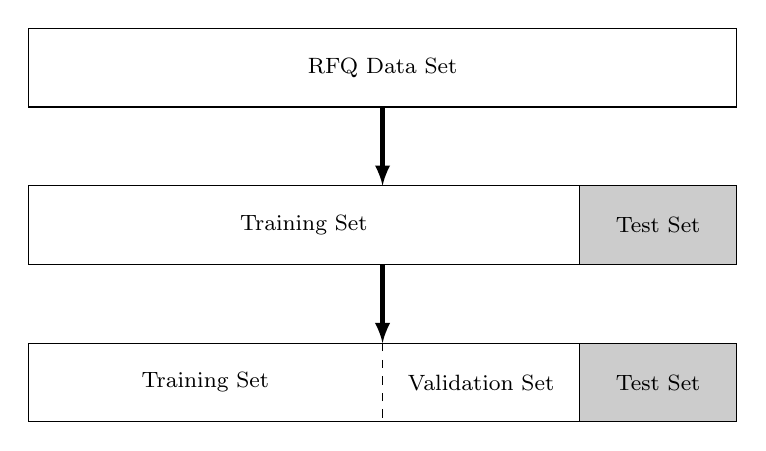
\begin{tikzpicture}[x=1cm,y=2cm]
        \begin{scope}[every node/.style={rectangle,minimum height=1cm,align=center,font=\footnotesize,anchor=west,inner sep=0pt,outer sep=0pt}]
            \node[text width=9cm,draw] (N1) at (0,0)  {RFQ Data Set};
            \node[text width=7cm,draw] (N21) at (0,-1) {Training Set};
            \node[text width=2cm,draw=black,fill=black!20] (N32) at (N21.east) {Test Set};
            \node[text width=4.5cm] (N31) at (0,-2) {Training Set};
            \node[text width=2.5cm] (N32) at (N31.east) {Validation Set};
            \node[text width=2cm,draw=black,fill=black!20] (N33) at (N32.east) {Test Set};
        \end{scope}
            \draw (N31.south west) rectangle (N32.north east);
            \draw[dashed] (N31.north east) rectangle (N31.south east);
        \begin{scope}[-latex,line width=1.5pt]
            \draw (N1.south) coordinate(X) -- (N21.north-|X);
            \draw (N21.south-|X) -- (N31.north-|X);
        \end{scope}
    \end{tikzpicture}
    \caption{Train-validation-test data split}\label{Ch1Fig:6}
\end{figure}

The models were evaluated on the training and validation portion of the data using `cross-validation', a process where hyperparameters are fine tuned. Hyperparameters are configurations external to the model (unlike model parameters) whose values cannot be learned from the data during the training process and are typically specified prior to training by machine learning practitioners. An example of a hyperparameter would be the learning rate for a neural network regression model (e.g. MLPregressor). The models were then retrained on the training set using the best hyperparameter thus returning the best model. The best model (with the optimal hyperparameters) is then run on the test data to see how well it generalises on the hitherto unseen test data. A detailed process map is provided in Section~\ref{train-testsplit}.


\section{Research Experiments}\label{Ch1Sec5}

The research experiments for this thesis are presented under three categories in Section~\ref{ch4:title}, in order of increasing complexity. They are designed to investigate predictability of RFQs using supervised and unsupervised models in both a Classical and Bayesian setting. \textbf{Experiments 1 and 2} attempt to predict RFQs using the selected supervised and unsupervised hidden Markov model respectively. More sophisticated insight is sought in \textbf{Experiment 3} by inferring the hidden ('latent') states of the RFQ market dynamics. This can be very insightful as it provides the ability to know at any point in time which type of regime the underlying market is operating in, for example: increasing, decreasing or level. 


\section{Thesis structure}\label{Ch1Sec5}

The structure of this thesis is organised as follows:

\begin{description}

\item[Chapter 1] -- Introduction. This chapter begins with providing the reader with the motivation for conducting this research. It highlights the validated business justification for this thesis as well as explaining why the timing is right. After which a very brief introduction to e-FX options, trading platforms and RFQs is provided based on intimate knowledge of financial markets. The chapter then highlights the research objectives and the overall methodology which includes RFQ data generation, model selection, model fitting and testing. Finally the chapter introduces the three experiments conducted in this thesis which cover prediction of RFQs as well as inferring the hidden states using the hidden Markov model.

\item[Chapter 2] -- Background and Literature Review. The aim of this chapter is to describe in detail key background concepts accompanied by relevant literature. It first presents the key role which machine learning plays in Finance and the expected impact it will have on the financial services industry. Thereafter a comprehensive review of Classical versus Bayesian philosophies is provided which includes a description of Bayes' Theorem. \\
This chapter then provides detailed coverage of the hidden Markov model (HMM) with precise definitions of relevant equations. After the HMM background and applications, belief networks are described, leading into Markov chains and subsequently the HMM. The iterative expectation maximisation (EM) algorithm is also covered in this chapter, both in the general form and specifically the Baum-Welch EM algorithm which is used by the HMM for learning.
Next, artificial neural networks are presented with key features and applications. Thereafter the focus is aimed at feed-forward type of neural networks which are relevant to this thesis. The chapter also covers their architecture, key components as well as the back-propagation and stochastic gradient descent, necessary for learning in a neural network.

\item[Chapter 3] -- RFQ Data Set. RFQ data generation of EUR-USD vanilla European options along with descriptive statistics is provided in this chapter. The 'binning' methodology for processing the RFQ data is presented and justified. The chapter also provides the reader with insight into the RFQ data using some key plots. Towards the end, the chapter describes the steps used to split the RFQ data for cross-validation, training and testing. The reader is also presented with data wrangling steps used to transform the RFQ data-set into a form suitable for consumption by each supervised and unsupervised model.

\item[Chapter 4] -- Experiments. To begin with, this chapter presents the overall model selection framework used for this thesis and the subsequent three experiments. Each experiment follows a similar format of: Introduction to the selected experiment and model, Model implementation, Results and discussion and finally a Conclusion. The experiments get progressively more sophisticated. \textbf{Experiment 1} begins with a brief introduction, the three selected supervised learning models are implemented, trained and evaluated in their ability to predict RFQs. \textbf{Experiment 2} creates and fits a hidden Markov model to make RFQ predictions using the most likely hidden state. This is demonstrated on both 1 (count) and 2 (count and notional) dimensional visible variables. The results for Experiment 2 are compared with those in Experiment 1. Finally, \textbf{Experiment 3} makes use of the hidden Markov model to make inferences about the underlying hidden ('latent') state of the RFQ market dynamics (e.g increasing, decreasing or level). The Viterbi algorithm is used to infer the most likely hidden path - the learning for this is done using the Baum-Welch iterative algorithm. This experiment also explains why a 'differences' methodology was adopted to transform the data into a Markovian state suitable for consumption by the hidden Markov model.

\item[Chapter 5 and 6] -- Conclusion and Further Work. The final 2 chapters provide the overall conclusion of this thesis as well as suggestions for further work.


\end{description}

%\textcolor{red}{TODO: Remove}
%\begin{conclusions}
%    This is the content of conclusions. Now it is in italic, but we will change the layout accordingly.
%\end{conclusions}